%% FGCS submission version (Elsevier elsarticle, 5p double-column).
%% Derived from paper-latex/ (IEEE version). Build:
%%   pdflatex main && bibtex main && pdflatex main && pdflatex main
\documentclass[5p,times,twocolumn,final]{elsarticle}

\usepackage[utf8]{inputenc}
\usepackage[T1]{fontenc}
\usepackage{graphicx}
\usepackage{amsmath,amssymb,amsthm}
\usepackage{booktabs}
\usepackage{multirow}
\usepackage{tabularx}
\usepackage{array}
\usepackage{xcolor}
\usepackage{caption}
\usepackage{subcaption}
\usepackage{url}
\usepackage[hidelinks]{hyperref}

\newtheorem{definition}{Definition}
\graphicspath{{./figures/}}
\captionsetup{font=small,labelfont=bf}
\captionsetup[sub]{font=footnotesize}

% Compact list environments
\newcommand{\squishlist}{\begin{itemize}\setlength{\itemsep}{1pt}\setlength{\parskip}{0pt}\setlength{\parsep}{0pt}}
\newcommand{\squishend}{\end{itemize}}
% Visible marker for items the authors must confirm before submission.
\newcommand{\authorcheck}[1]{\textcolor{red}{[CHECK: #1]}}

\journal{Future Generation Computer Systems}

\begin{document}

\begin{frontmatter}

\title{Blockchain Data Availability: Benchmarking Throughput, Economics, Utilization, and Security of Six Production Protocols}

\author[cs]{Prasad Kumkar\corref{cor1}}
\ead{prasad@chainscorelabs.com}
\author[cs]{Pranjal Sarode}
\ead{pranjal@chainscorelabs.com}
\cortext[cor1]{Corresponding author.}
\affiliation[cs]{organization={Chainscore Labs},
            city={Pune},
            state={Maharashtra},
            country={India}}

\begin{abstract}
Data availability (DA) is a critical bottleneck in blockchain scalability.
This paper presents a benchmarking study of six production DA protocols (Polkadot ELVES, Ethereum EIP-4844/PeerDAS, Celestia, Espresso Tiramisu, NEAR, and Avail) using 90 days of mainnet data (November 2025 to February 2026).
We introduce a taxonomy that classifies DA architectures into three paradigms: data availability sampling (DAS), verifiable information dispersal (VID), and validator-set recovery.
Under a unified methodology we measure throughput (MiB/s), cost (\$/MiB), utilization, and block dynamics across all six protocols.
Key findings are: (i)~mean utilization stays below 40\% for every protocol, so current measurements are demand-constrained rather than supply-constrained; (ii)~median DA cost spans more than eight orders of magnitude, from nano-dollars (Espresso) to tens of cents per MiB (NEAR); (iii)~no protocol slashes for pure data withholding, so enforcement is indirect in every design; and (iv)~no protocol guarantees permanent availability: protocol-defined retention ranges from $\sim$25~hours (Polkadot) to $\sim$18~days (Ethereum), while Avail and Espresso leave retention to node operators.
Ethereum's Fusaka upgrade and two blob-parameter-only forks fall inside the window and serve as natural experiments on fee-market behaviour.
We release all collection tooling, datasets, and analysis code under open licenses.
\end{abstract}

\begin{keyword}
data availability \sep blockchain scalability \sep erasure coding \sep data availability sampling \sep benchmarking \sep rollups \sep distributed systems \sep measurement
\end{keyword}

\end{frontmatter}

% ================================================================
\section{Introduction}
\label{sec:introduction}
% ================================================================
% SECTION I: INTRODUCTION
% ================================================================

A blockchain can scale only if every participant can be confident that block data has been published and can be retrieved.
This property, \emph{data availability} (DA), is a security requirement for rollups, parachains and sharded designs.
Without it, validators cannot verify state transitions, light clients cannot detect fraud, and the system's trust model reduces to that of a permissioned committee~\cite{Saif_Survey_DA_Rollups}.

Several DA designs have reached production in the past three years.
Ethereum introduced blob-carrying transactions (EIP-4844) and, with the Fusaka upgrade in December 2025, activated PeerDAS for cell-level sampling~\cite{EIP-4844, EIP-7594}.
Celestia launched the first dedicated DA network with two-dimensional erasure coding and namespace-filtered sampling~\cite{AlBassam_LazyLedger}.
Polkadot's ELVES protocol distributes erasure-coded parachain data across its validator set with approval-gated finality~\cite{Jeff_Burdges_ELVES}.
Espresso's Tiramisu introduces a three-layer Verifiable Information Dispersal (VID) architecture that explicitly rejects DAS in favor of algebraic dispersal proofs~\cite{Espresso:Hotshot_and_Triamisu}.
NEAR provides sharding-based DA through Nightshade with a rollup-oriented blob store~\cite{NEAR_Nightshade_Scaling_Blockchain}, and Avail combines KZG polynomial commitments with DAS-enabled light clients on a Substrate-based chain~\cite{Avail_The_DA_Blockchain}.

Published comparisons of these designs are qualitative surveys~\cite{Saif_Survey_DA_Rollups, Thibault2022Rollups}, vendor material, or measurements of a single protocol~\cite{Heimbach2025BlobFee, Lee2025BlobSharing}.
We are not aware of a study that measures throughput, cost and utilization across several DA networks with one methodology, so rollup developers choosing a DA backend have no common empirical baseline to work from.

This paper makes the following contributions:

\begin{enumerate}
    \item A taxonomy that classifies DA protocols by verification paradigm (data availability sampling, verifiable information dispersal, or validator-set recovery), encoding scheme and commitment type (Section~\ref{sec:background}).

    \item A comparison of encoding redundancy, commitment schemes (KZG, NMT and Merkle) and verification mechanisms across the six protocols, based on their specifications and documentation (Section~\ref{sec:architecture}).

    \item Measurements from 90~days of mainnet data (November 2025--February 2026) for Polkadot, Ethereum, Celestia, Espresso, NEAR and Avail, covering throughput (MiB/s), cost (\$/MiB), utilization and block dynamics under common definitions (Section~\ref{sec:results}).

    \item A comparison of trust assumptions, Byzantine fault tolerance thresholds, withholding enforcement and retention policies (Section~\ref{sec:security}).

    \item The collection scripts, raw datasets and analysis code, released under Apache~2.0 (code) and CC~BY~4.0 (data).
\end{enumerate}


\section{Background and Related Work}
\label{sec:background}
% ================================================================
% SECTION II: BACKGROUND AND RELATED WORK
% ================================================================

% ------------------------------------------------------------------
% II-A. Data Availability Fundamentals
% ------------------------------------------------------------------
\subsection{Data Availability Fundamentals}
\label{subsec:da-fundamentals}

Data availability (DA) must be distinguished from the related but distinct problems of data \emph{storage} and data \emph{retrieval}.
Storage concerns the persistence of data over time; retrieval concerns the ability to read stored data on demand.
DA addresses a different question: \emph{was the data published at all?}
Formally, a block producer who withholds part of a block's data can cause validators and light clients to accept an invalid state transition, because the withheld data may contain a fraudulent transaction whose invalidity can never be proven if the data is unavailable~\cite{AlBassam_FraudDA}.

\begin{definition}[Data Availability]
A block $B$ satisfies the data availability property if every honest participant can retrieve the complete block data within a bounded time window $\Delta$ after the block header is published.
\end{definition}

A DA scheme must provide four properties:

\begin{enumerate}
    \item \textbf{Completeness.} All data constituting block $B$ is published to the network. A DA scheme is complete if no honest node accepts a block header unless the corresponding data has been made available to the network.

    \item \textbf{Soundness.} The encoding of $B$ is verifiably correct. Given a commitment $C(B)$ included in the block header, any participant can verify that a received coded piece is consistent with $C(B)$ without possessing the entire block.

    \item \textbf{Availability detection.} Resource-constrained participants (light clients) can assess whether the data behind a block header is available without downloading the full block. This property separates DA from simple data retrieval.

    \item \textbf{Reconstruction.} The original data $B$ can be recovered from any sufficiently large subset of coded pieces. If $E(B)$ denotes the erasure-coded encoding of $B$ producing $n$ coded pieces with redundancy factor $r$, then $B$ is reconstructible from any $n/r$ pieces.
\end{enumerate}

\noindent\textbf{Notation.}
Throughout this paper we use the following conventions.
A block's raw data is denoted $B$, with $|B|$ its size in bytes.
The encoding function $E(B)$ produces $n$ coded pieces (variously called shares, chunks, or cells depending on the protocol).
A commitment $C(B)$ is included in the block header and serves as a binding digest of $E(B)$.
Verification $V(C, s_i)$ checks that coded piece $s_i$ is consistent with commitment $C$.
The redundancy factor $r = n \cdot |s_i| / |B|$ captures the total storage expansion introduced by the encoding.


% ------------------------------------------------------------------
% II-B. Taxonomy of DA Approaches
% ------------------------------------------------------------------
\subsection{Taxonomy of DA Approaches}
\label{subsec:taxonomy}

We classify the six protocols along three dimensions: the \emph{availability verification paradigm} (how clients gain confidence that data is available), the \emph{encoding scheme} (how raw data is expanded into coded pieces: 1D Reed--Solomon~\cite{Reed1960RS}, 2D Reed--Solomon, or polynomial VID), and the \emph{commitment scheme} (how pieces are bound to the header: KZG~\cite{KZG_Original}, Namespaced Merkle Trees, or plain Merkle trees).
Section~\ref{sec:architecture} compares encodings and commitments in detail; here we define the three verification paradigms.

\paragraph{DAS (Avail, Celestia, Ethereum/PeerDAS)}
Light clients request a few random coded pieces; if all arrive with valid proofs, the client concludes with high probability that the full data is available.
Security rests on an \emph{honest-minority} assumption: at least one honest, non-eclipsed full node must seed correctly encoded pieces into the network.

\paragraph{Validator-set recovery (Polkadot, NEAR)}
The validator set collectively stores erasure-coded chunks and attests to availability through consensus (Polkadot's availability bitfields~\cite{Jeff_Burdges_ELVES}, NEAR's per-shard chunk producers~\cite{NEAR_Nightshade_Scaling_Blockchain}); there is no client-side sampling.

\paragraph{VID (Espresso)}
Verifiable information dispersal~\cite{Cachin2005AVID} combines erasure coding with algebraic proofs that each committee member received a valid piece; a threshold of signatures forms a DA certificate~\cite{Espresso:Hotshot_and_Triamisu}.
Light-client confidence derives from the certificate, not from sampling.

\subsection{Protocols Under Study}
\label{subsec:protocol-descriptions}

We summarize each protocol as deployed during our window (November 2025--February 2026); Table~\ref{tab:feature_comparison} gives the parameters.

\paragraph{Polkadot (ELVES)}
The relay chain erasure-codes parachain Proof-of-Validity (PoV) data across $\sim$600 validators~\cite{Jeff_Burdges_ELVES, Overview_of_polkadot}; a block is available once two-thirds sign availability bitfields, after which it enters approval checking and GRANDPA finality.
Up to 100~cores each carry a PoV of up to 10~MiB every 6~s. DA is priced through coretime rather than per byte, and chunks are kept for $\sim$25~hours.

\paragraph{Ethereum (EIP-4844 and PeerDAS)}
Blobs of 128~KiB are committed with KZG and priced by a separate exponential blob-gas market~\cite{EIP-4844}.
Pectra (EIP-7691~\cite{EIP-7691}) set a target/maximum of 6/9 blobs per block.
The Fusaka upgrade on 3~December 2025 activated PeerDAS (EIP-7594~\cite{EIP-7594}), with 2$\times$ column extension over 128 columns, and EIP-7918~\cite{EIP-7918}, which bounds the blob base fee from below by a fraction of the execution base fee.
Two blob-parameter-only (BPO) forks then raised the target/maximum to 10/15 (9~December) and 14/21 (7~January 2026).
Blobs are pruned after 4{,}096 epochs ($\sim$18~days).

\paragraph{Celestia}
A $k \times k$ original data square is extended to $2k \times 2k$ and committed with Namespaced Merkle Trees, enabling namespace-filtered retrieval~\cite{AlBassam_LazyLedger}.
CometBFT gives single-slot finality every $\sim$6~s. App version~6 activated on 24~November 2025, and on 3~December the maximum square rose from $128 \times 128$ (8~MiB) to $256 \times 256$ (32~MiB). Light nodes sample within a 7-day window (CIP-036).

\paragraph{Espresso (Tiramisu)}
Tiramisu layers a KZG-based VID scheme (Savoiardi), a DA committee for fast retrieval (Mascarpone), and an untrusted CDN for bulk delivery~\cite{Espresso:Hotshot_and_Triamisu}; it is now marketed as EspressoDA.
HotShot gives responsive finality of $\sim$2~s and the maximum block size was 1~MB throughout our window. Mainnet~0 runs 100~nodes operated by 20~parties without slashing. Retention is set per node: pruning is off by default and, when enabled, targets 7~days.

\paragraph{NEAR}
Nightshade shards erasure-code chunk data among each shard's chunk producers~\cite{NEAR_Nightshade_Scaling_Blockchain}.
Rollups post data as function-call input to a blob-store contract; it is pruned after the 5-epoch garbage-collection window ($\sim$1.5~days at the $\sim$0.6~s block time in force since May 2025). A single transaction is capped at 1.5~MiB. There is no DAS and no active withholding challenge.

\paragraph{Avail}
Row-wise 1D Reed--Solomon encoding with KZG commitments supports DAS by light clients over a DHT~\cite{Avail_The_DA_Blockchain}.
BABE/GRANDPA produce a block every 20~s; application-specific data retrieval lets clients download only their application's data.
The maximum block size was 4~MiB throughout the window. Nodes prune \emph{state} after 256~blocks but keep block data by default, so there is no protocol-defined DA expiry; the VectorX bridge relays DA attestations to Ethereum with a $\sim$2-hour delay.


% ------------------------------------------------------------------
% II-D. Related Work
% ------------------------------------------------------------------
\subsection{Related Work}
\label{subsec:related-work}

\paragraph{Foundational theory}
Croman et al.~\cite{Croman2016Scaling} quantified the throughput and latency limits of monolithic blockchains, motivating the separation of data publication from execution.
Al-Bassam et al.~\cite{AlBassam_FraudDA} introduced fraud and data availability proofs, the foundation for DAS: by erasure-coding block data and letting light clients randomly sample coded pieces, a network can guarantee availability with high probability under an honest-minority assumption.
Hall-Andersen, Simkin, and Wagner formalized the security definition of DAS~\cite{HallAndersen2025FoundationsDAS} and proposed FRIDA, a DAS construction without a trusted setup~\cite{HallAndersen2024FRIDA}.
Coded Merkle Trees~\cite{Yu2020CodedMerkle} and the ACeD oracle~\cite{Sheng2021ACeD} reduce the cost of detecting incorrect coding.
On the dispersal side, asynchronous verifiable information dispersal~\cite{Cachin2005AVID} is the primitive behind committee-based designs, and Nazirkhanova, Neu, and Tse~\cite{Nazirkhanova2022VID} adapted it to rollups using KZG commitments~\cite{KZG_Original}; Fisch et al.~\cite{Fisch2025PermissionlessVID} extend VID to permissionless settings.

\paragraph{Protocol-specific designs}
Al-Bassam's LazyLedger proposal~\cite{AlBassam_LazyLedger} introduced a dedicated DA blockchain with namespace-filtered retrieval, which evolved into Celestia.
Burdges et al.~\cite{Jeff_Burdges_ELVES} formalized Polkadot's ELVES protocol for availability and validity, proving security under Byzantine assumptions with approval-based checking.
Bearer et al.~\cite{Espresso:Hotshot_and_Triamisu} describe the HotShot consensus and Tiramisu DA architecture.
Ethereum has progressed from blob transactions (EIP-4844~\cite{EIP-4844}) through blob throughput increases (EIP-7691~\cite{EIP-7691}) to peer-level DAS (EIP-7594~\cite{EIP-7594}), an incremental path toward Danksharding~\cite{Buterin_Danksharding}; Chaudhuri et al.~\cite{CodexDAS} and Pigaglio et al.~\cite{Pigaglio2025PANDAS} study the networking design space of Ethereum DAS through simulation.

\paragraph{Empirical and economic studies}
Several recent studies measure Ethereum's blob market in isolation.
Crapis et al.~\cite{Crapis2024EIP4844Econ} model the economics of EIP-4844; Heimbach et al.~\cite{Heimbach2025BlobFee} and Park et al.~\cite{Park2026EIP4844Impact} analyse blob fee dynamics and the impact of EIP-4844; and Lee et al.~\cite{Lee2025BlobSharing} measure blob utilisation over 180~days.
All of these focus on Ethereum alone.

\paragraph{Surveys}
Saif et al.~\cite{Saif_Survey_DA_Rollups} and Thibault et al.~\cite{Thibault2022Rollups} survey DA and rollup designs, classifying approaches by trust assumptions and encoding strategies, without measurements from production networks.

\paragraph{Positioning of this work}
To our knowledge, this paper is the first to measure six production DA protocols simultaneously under one methodology.
Prior empirical work covers Ethereum alone, and prior comparative work is qualitative or simulation-based.
Our study complements the theoretical results above and the surveys of~\cite{Saif_Survey_DA_Rollups, Thibault2022Rollups} by providing a cross-protocol empirical baseline, and it is the first to observe Ethereum's DA market across the Fusaka (PeerDAS) and BPO transitions.


\section{Protocol Architecture Comparison}
\label{sec:architecture}
% ================================================================
% SECTION III: PROTOCOL ARCHITECTURE COMPARISON
% ================================================================

We compare the six protocols on encoding and redundancy, commitment scheme, and verification paradigm.
These choices fix a protocol's bandwidth cost, what a light client can check on its own, and which parties must be trusted.

% ----------------------------------------------------------
% III-A. ENCODING AND REDUNDANCY
% ----------------------------------------------------------
\subsection{Encoding and Redundancy}
\label{subsec:encoding}

All six protocols use Reed--Solomon (RS) erasure coding, but they differ in dimensionality, redundancy factor and how data is reconstructed.
Table~\ref{tab:encoding_comparison} summarizes these differences.

\begin{table}[t]
\centering
\caption{Encoding and redundancy.}
\label{tab:encoding_comparison}
\setlength{\tabcolsep}{2pt}
\footnotesize
\begin{tabular}{l l c l}
\toprule
\textbf{Protocol} & \textbf{Encoding} & \textbf{Redund.} & \textbf{Reconstruction} \\
\midrule
Polkadot~\cite{Jeff_Burdges_ELVES} & 1D RS (validators) & ${\sim}3\times$ & $f{+}1$ of $n$ ($n{=}3f{+}k$) \\
Ethereum~\cite{EIP-7594} & 1D RS (PeerDAS cells) & ${\sim}2\times$ & 50\%+ of 128 columns \\
Celestia~\cite{AlBassam_LazyLedger} & 2D RS ($k \times k \to 2k \times 2k$) & ${\sim}4\times$ & $k{\times}k$ shares \\
Espresso~\cite{Espresso:Hotshot_and_Triamisu} & Polynomial VID & $1/r$, $r{=}m/n$ & $m$ of $n$ evaluations \\
NEAR~\cite{NEAR_Nightshade_Scaling_Blockchain} & 1D RS (chunk parts) & ${\sim}3\times$ & $1/3$ of parts \\
Avail~\cite{Avail_The_DA_Blockchain} & 1D RS (row-wise) & ${\sim}2\times$ & $n$ of $2n$ coded pieces \\
\bottomrule
\end{tabular}
\end{table}

Higher redundancy costs proportionally more bandwidth and aggregate storage; in return, data can be recovered when a larger fraction of coded pieces is missing.

Celestia has the highest redundancy at ${\sim}4\times$ due to its two-dimensional RS structure: original data of dimension $k \times k$ is extended to $2k \times 2k$, yielding four times the original data volume in shares~\cite{AlBassam_LazyLedger}.
The overhead pays for two-dimensional sampling, in which light clients sample from both the rows and the columns of the extended matrix.
The 2D layout also allows a single row or column of length $2k$ to be recovered from any $k$ of its shares, so a node can repair one row without reconstructing the whole block.

Polkadot and NEAR both use ${\sim}3\times$ redundancy, distributing erasure-coded pieces across their respective validator sets.
In Polkadot's ELVES protocol, parachain block data (Proofs of Validity, or PoVs) are RS-encoded and distributed such that each validator stores one coded chunk, with reconstruction requiring $f{+}1$ of $n$ chunks where $n = 3f + k$~\cite{Jeff_Burdges_ELVES, Overview_of_polkadot}.
NEAR's Nightshade sharding similarly encodes chunk data with ${\sim}3\times$ redundancy, requiring only $1/3$ of the parts for reconstruction~\cite{NEAR_Nightshade_Scaling_Blockchain}.
In both, responsibility for the data is spread over the validator set; there is no separate committee and no sampling.

Ethereum and Avail have the lowest redundancy, ${\sim}2\times$.
Ethereum's EIP-4844 blob transactions encode data into 128-byte cells arranged across 128 columns. PeerDAS extends each blob's polynomial evaluation points such that any 64 of the 128 columns suffice for reconstruction~\cite{EIP-7594}.
Avail performs row-wise RS encoding on its application data matrix, extending $n$ original pieces to $2n$ coded pieces per row, so that any $n$ of the $2n$ pieces suffice for recovery~\cite{Avail_The_DA_Blockchain}.
With a $2\times$ extension any half of the coded pieces recovers the data, which together with KZG commitments is enough for DAS.

Espresso's Tiramisu uses a polynomial-based verifiable information dispersal (VID) scheme.
Data is represented as a polynomial that is evaluated at $n$ distinct points (one per committee member); any $m$ evaluations suffice for interpolation, where the code rate $r = m/n$ is configurable~\cite{Espresso:Hotshot_and_Triamisu}.
Algebraically this is an RS code, but because it is built into the VID commitment layer, one proof certifies both that the encoding is correct and that each member received its piece.

% ----------------------------------------------------------
% III-B. COMMITMENT SCHEMES AND PROOF SYSTEMS
% ----------------------------------------------------------
\subsection{Commitment Schemes and Proof Systems}
\label{subsec:commitments}

The commitment scheme determines what a light client can verify, whether a trusted setup is needed, and the cost of producing and checking proofs.
The six protocols use three families: KZG polynomial commitments, Namespaced Merkle Trees (NMTs) and standard Merkle trees.
Table~\ref{tab:commitment_comparison} compares their properties.

\begin{table}[t]
\centering
\caption{Commitment scheme properties (KZG: Avail, Ethereum, Espresso; NMT: Celestia; Merkle: Polkadot, NEAR).}
\label{tab:commitment_comparison}
\setlength{\tabcolsep}{2pt}
\footnotesize
\begin{tabular}{l c c c}
\toprule
\textbf{Property} & \textbf{KZG} & \textbf{NMT} & \textbf{Merkle} \\
\midrule
Proof size & $O(1)$, ${\sim}48$ bytes & $O(\log n)$ & $O(\log n)$ \\
Trusted setup & Yes (SRS) & No & No \\
Namespace filter & No & Native & No \\
Verification & Pairings & Hashes & Hashes \\
Encoding correctness & Algebraic & Fraud proofs & Not verifiable \\
\bottomrule
\end{tabular}
\end{table}

KZG polynomial commitments~\cite{KZG_Original} are used by Avail, Ethereum, and Espresso.
A KZG commitment to a polynomial $p(x)$ of degree $d$ is a single elliptic curve group element (${\sim}48$ bytes on BLS12-381), and an opening proof for any evaluation $p(z) = v$ is also a single group element.
Verification requires two pairing operations, which are computationally more expensive than hash evaluations but yield $O(1)$-size proofs regardless of the data size.
KZG commitments enable \emph{algebraic verification of encoding correctness}: given commitments to the rows (or columns) of an erasure-coded data matrix, anyone can verify that the extended portions are consistent with the original data by checking polynomial relationships between commitments, without accessing the underlying data.
This lets Avail and Ethereum light clients reject incorrectly encoded data without fraud proofs.
The drawback is that KZG needs a structured reference string (SRS) from a trusted setup; anyone holding the setup's secret could forge proofs.
Ethereum and Avail both ran multi-party ceremonies to reduce this risk, Ethereum's with over 140{,}000 contributors.

Celestia uses Namespaced Merkle Trees (NMTs)~\cite{AlBassam_LazyLedger}.
An NMT is a standard Merkle tree augmented with namespace identifiers: each leaf is tagged with a namespace, internal nodes carry the minimum and maximum namespace of their subtrees, and the tree is sorted by namespace.
This structure enables \emph{namespace inclusion and exclusion proofs}. A light client can request all shares belonging to a specific namespace (e.g., a particular rollup's data) and receive a Merkle proof that the returned set is complete (no shares from that namespace have been omitted, and no extraneous shares have been included).
Rollup nodes use this to download only their own data instead of the whole block.
NMT proofs are $O(\log n)$ in size.
Encoding correctness, however, is \emph{not} algebraically verifiable from the NMT alone. Instead, Celestia relies on Bad Encoding Fraud Proofs (BEFPs) to detect and propagate evidence of incorrect erasure coding~\cite{AlBassam_FraudDA}.

Polkadot and NEAR use standard Merkle trees.
Polkadot commits to erasure-coded PoV chunks via a Merkle trie whose root is included in the relay chain block header~\cite{Overview_of_polkadot, polkadot_article}.
NEAR similarly uses Merkle roots to commit to chunk data within shard blocks.
Merkle inclusion proofs are $O(\log n)$ and need only hashing to verify.
They give light clients no way to check encoding correctness or to sample: a proof shows that a piece belongs to the committed set but says nothing about whether the erasure coding was done correctly.
In both Polkadot and NEAR, encoding correctness is enforced through the validator set (validators who reconstruct and re-encode can detect errors), but this verification is not accessible to light clients or external observers.

% ----------------------------------------------------------
% III-C. VERIFICATION PARADIGMS
% ----------------------------------------------------------
\subsection{Verification Paradigms: DAS, VID, and Validator Recovery}
\label{subsec:verification}

The protocols differ most in how availability is verified.
The three paradigms below differ in their trust assumptions and in what a light client can check.

% --- DAS ---
\subsubsection{Data Availability Sampling (DAS)}

DAS, as formalized by Al-Bassam et al.~\cite{AlBassam_FraudDA}, enables light clients to verify data availability without downloading the full block.
A light client randomly requests $s$ coded pieces from the network; if all $s$ are returned, the client gains probabilistic confidence that the full data is available.
Against a $(1{-}q)$-withholding adversary (one that has made fraction $q$ of the data unavailable), a client sampling $s$ independent pieces achieves confidence $1 - q^s$.

Celestia was the first production network to deploy DAS.
Its 2D RS structure means that light clients sample from the $2k \times 2k$ extended square.
Because an adversary must withhold at least ${\sim}25\%$ of the extended square to prevent reconstruction, each sample detects withholding with probability ${\ge}1/4$, so 16 random samples give a Celestia light client approximately $1 - (3/4)^{16} \approx 99\%$ confidence that the data is available, assuming that at least one honest full node is non-eclipsed and participates in the peer-to-peer network~\cite{AlBassam_LazyLedger}.

Avail implements DAS over its 1D RS-encoded rows with KZG commitments.
Avail light clients sample random cells from the data matrix; each cell is accompanied by a KZG opening proof.
With 10 random samples, an Avail light client achieves $1 - (1/2)^{10} \approx 99.9\%$ confidence ($1 - 1/1024$)~\cite{Avail_The_DA_Blockchain}.
Because each cell is checked against the committed row polynomial, the client also verifies encoding correctness without fraud proofs.
Avail light clients fetch cells from a Kademlia DHT run by light clients and fall back to full-node RPC; cells fetched over RPC are written back into the DHT, so later requests can be served by other light clients.

Ethereum activated DAS through PeerDAS (EIP-7594) in the Fusaka upgrade on 3~December 2025.
Under PeerDAS, each blob is extended from 64 to 128 evaluation points (columns), and each validator is responsible for custody of a subset of columns determined by its node ID.
In the Fulu specification every node custodies at least 4 of 128 custody groups (\texttt{CUSTODY\_REQUIREMENT}), nodes with attached validators custody at least 8 plus one per 32~ETH of balance (\texttt{VALIDATOR\_CUSTODY\_REQUIREMENT}), and every node samples 8 columns per slot (\texttt{SAMPLES\_PER\_SLOT})~\cite{EIP-7594}.
Each node samples only a few columns, so confidence comes from the aggregate: with custody spread over ${\sim}1{,}000{,}000$ validators, each of the 128 columns is very likely held by at least one honest validator.
PeerDAS also introduces a ``supernode'' role: nodes that subscribe to all 128~data column subnets and can reconstruct the full data matrix from partial columns. The Fulu networking specification requires at least one supernode on the network for reconstruction of missing data, an assumption that did not exist before PeerDAS, when every consensus node downloaded all blob data~\cite{EIP-7594}.

DAS on all three protocols relies on two assumptions: (i)~at least one honest, non-eclipsed full node must hold the complete data and respond to sampling requests, and (ii)~sufficient sampling participation must exist in the network to ensure that withholding is detected before the data propagation window closes.
An adversary capable of eclipsing a light client's peer connections can cause the client to falsely conclude that data is available (or unavailable) regardless of the true state.

% --- Validator-Set Recovery ---
\subsubsection{Validator-Set Recovery}

In Polkadot and NEAR the validator set stores and serves the erasure-coded data, and availability is attested through consensus instead of sampling.

Polkadot's ELVES protocol ties availability to finality~\cite{Jeff_Burdges_ELVES}.
After a parachain collator produces a block candidate, the relay chain validators erasure-code the Proof of Validity (PoV) and distribute one chunk per validator.
Each validator that successfully receives and stores its chunk signs an \emph{availability bitfield} (a bitmap indicating which PoV chunks it holds).
A PoV is considered available when $\geq 2/3$ of validators have signed its bitfield.
The GRANDPA finality gadget will not finalize a relay chain block unless the availability bitfields for all included parachain candidates have reached the $2/3$ threshold~\cite{Overview_of_polkadot, polkadot_article}.
Under the $2/3$ honest-majority assumption the guarantee is deterministic: unavailable data cannot be finalized.

NEAR's Nightshade sharding distributes chunk data across shard validators (chunk producers).
Each chunk producer is responsible for producing and serving the chunk parts for its assigned shard.
NEAR's availability enforcement relies on a ``lazy signer'' mechanism with probabilistic accountability: validators are required to attest to chunk availability, but enforcement is primarily through the consensus protocol's liveness requirements rather than explicit sampling~\cite{NEAR_Nightshade_Scaling_Blockchain}.
A challenge mechanism exists in the block structure for disputing invalid or unavailable chunks, but as of our observation period, this mechanism is ``not used today'' in practice.

Because availability evidence is a precondition for finality (Polkadot) or block production (NEAR), validators have a direct incentive to store and serve data.
Light clients, however, cannot check availability themselves: a Polkadot or NEAR light client must trust that the $\geq 2/3$ supermajority attested honestly, with only the validators' stake behind that trust.

% --- VID ---
\subsubsection{Verifiable Information Dispersal (VID)}

Espresso's Tiramisu replaces DAS with algebraic dispersal proofs~\cite{Espresso:Hotshot_and_Triamisu}.
It has three layers:

\squishlist
\item \textbf{Savoiardi (VID layer):} Data is encoded as a polynomial and evaluated at $n$ points (one per committee member). A vector commitment (using KZG) binds the evaluations to the polynomial commitment, producing a compact proof that each committee member received a correct evaluation. This provides \emph{bribery resistance}: even if an adversary bribes a threshold of committee members, the algebraic binding prevents them from claiming to hold data they do not possess.

\item \textbf{Mascarpone (certification layer):} Committee members who receive and verify their evaluations produce threshold signatures attesting to availability. A DA certificate is formed when $\geq 2/3$ of the committee has signed, providing a compact ($O(1)$-size) availability attestation.

\item \textbf{Cocoa (CDN layer):} A secondary retrieval path through an untrusted CDN that provides availability even if committee members go offline, with cryptographic proofs linking the fallback data to the original VID commitments.
\squishend

Confidence is deterministic: there is no sampling, and a block is finalized only with a DA certificate.
DAS detects withholding probabilistically, whereas Savoiardi's algebraic binding makes it infeasible for a committee member to claim falsely that it holds its piece.

Retrieval, however, requires cooperation from the committee or the Cocoa CDN.
There is no mechanism for an independent light client to sample data and verify availability without relying on the committee's attestations.
Espresso argues that DAS adds ``unnecessary redundancies'' given VID's algebraic guarantees~\cite{Espresso:Hotshot_and_Triamisu}; as a result, retrievability depends on the committee and the CDN.

% ----------------------------------------------------------
% CROSS-CUTTING: WITHHOLDING ENFORCEMENT
% ----------------------------------------------------------
\subsubsection{No Slashing for Data Withholding}

None of the six protocols slashes for pure data withholding.
Each has some way to detect or discourage it, but enforcement is always indirect:

\squishlist
\item \textbf{Polkadot:} Validators are slashed for casting invalid \emph{validity} votes (attesting that an invalid parachain block is valid), but there is no slashing for failing to store or serve erasure-coded chunks. A validator that withholds its chunk simply does not sign the availability bitfield, potentially delaying but not corrupting finality~\cite{Jeff_Burdges_ELVES}.

\item \textbf{Celestia:} Bad Encoding Fraud Proofs (BEFPs) allow any full node to prove that the block producer performed incorrect erasure coding~\cite{AlBassam_FraudDA}. However, BEFPs address encoding correctness, not data withholding. A block producer that correctly encodes data but subsequently withholds it faces no direct slashing penalty.

\item \textbf{Ethereum:} PeerDAS enforces availability through peer scoring and disconnection: validators that fail to serve their custody columns receive negative gossip scores and may be disconnected from the p2p network. There is no protocol-level slashing for custody failures~\cite{EIP-7594}.

\item \textbf{Espresso:} In the current Mainnet~0 deployment, enforcement is reputational only. No slashing mechanism is implemented for committee members that fail to serve their VID evaluations~\cite{Espresso:Hotshot_and_Triamisu}.

\item \textbf{NEAR:} A challenge mechanism exists in the block structure that would allow validators to dispute chunk unavailability, but this mechanism is ``not used today'' in the production network. Enforcement relies on the consensus protocol's liveness requirements~\cite{NEAR_Nightshade_Scaling_Blockchain}.

\item \textbf{Avail:} Slashing is implemented for equivocation (double-signing) but not for data withholding. Validators that fail to make sampled cells available face no direct economic penalty~\cite{Avail_The_DA_Blockchain}.
\squishend

Proving that a node \emph{has} data but \emph{refuses} to serve it is harder than proving that it served \emph{incorrect} data.
Withholding is an omission fault, and attributing an omission to malice instead of a network partition, latency or node failure is an open problem in distributed systems.

% ----------------------------------------------------------
% COMPREHENSIVE FEATURE COMPARISON TABLE
% ----------------------------------------------------------

\begin{table*}[t]
\centering
\caption{Feature and parameter comparison of the six DA protocols during the observation window.}
\label{tab:feature_comparison}
\setlength{\tabcolsep}{1.8pt}
\renewcommand{\arraystretch}{1.15}
\footnotesize
\begin{tabular}{l c c c c c c}
\toprule
\textbf{Feature} & \textbf{Polkadot} & \textbf{Ethereum} & \textbf{Celestia} & \textbf{Espresso} & \textbf{NEAR} & \textbf{Avail} \\
\midrule
Encoding &
  1D RS (validators) &
  1D RS (PeerDAS) &
  2D RS ($k{\to}2k$) &
  Poly.\ VID &
  1D RS (chunks) &
  1D RS (rows) \\
Commitment &
  Merkle trie &
  KZG &
  NMT &
  KZG + vector &
  Merkle &
  KZG \\
Redundancy &
  ${\sim}3\times$ &
  ${\sim}2\times$ &
  ${\sim}4\times$ &
  Configurable &
  ${\sim}3\times$ &
  ${\sim}2\times$ \\
DAS support &
  No &
  Yes (PeerDAS) &
  Yes (2D) &
  No (VID) &
  No &
  Yes (1D) \\
Light client DAS &
  No &
  Custody &
  Yes (16 samples) &
  No &
  No &
  Yes (10 samples) \\
Block time &
  6\,s (relay) &
  12\,s &
  6\,s &
  ${\sim}2$\,s &
  ${\sim}0.6$\,s &
  20\,s \\
Max DA capacity &
  10\,MiB$\times$100 &
  2.63\,MiB (BPO2) &
  8$\to$32\,MiB$^\ast$ &
  ${\sim}1$\,MiB &
  4\,MiB$\times$9 &
  4\,MiB \\
Protocol max MiB/s & $\sim$167 & $\sim$0.22 & 1.33$\to$5.31$^\ast$ & $\sim$0.37 & $\sim$59 & $\sim$0.21 \\
Finality &
  12--60\,s &
  ${\sim}13$\,min &
  ${\sim}6$\,s &
  ${\sim}2$\,s &
  ${\sim}2$\,s &
  20--60\,s \\
DA retention &
  25\,h &
  ${\sim}18$\,d &
  7\,d (sampling) &
  Node-set &
  ${\sim}1.5$\,d &
  Node-set$^\dagger$ \\
Fee model &
  Weight-based &
  Blob market &
  Gas-based &
  Per-byte &
  Gas-based &
  Weight-based \\
Withholding &
  Finality gate &
  Peer scoring &
  BEFPs (encoding) &
  Reputational &
  Unused challenge &
  None \\
Byzantine threshold &
  $f < n/3$ &
  $f < n/3$ &
  $f < n/3$ &
  $f < n/3$ &
  $f<n/3$/shard &
  $f < n/3$ \\
\bottomrule
\end{tabular}

\vspace{2pt}
\raggedright\footnotesize{$^\ast$Celestia's maximum square rose from 128 to 256 (8 to 32~MiB) on 3~Dec~2025. $^\dagger$Avail prunes state after 256 blocks, but block data is kept by default (Substrate \texttt{archive-canonical} block pruning).}
\end{table*}

Table~\ref{tab:feature_comparison} collects these parameters.
DAS protocols (Celestia, Avail, and Ethereum with PeerDAS) let light clients verify availability themselves but depend on network-level assumptions; validator-recovery (Polkadot, NEAR) and VID (Espresso) designs give deterministic guarantees that hold only if the validators or committee are honest.
The commitment scheme follows from the paradigm: KZG gives Ethereum, Avail and Espresso algebraic encoding checks, Celestia pairs sampling with NMTs and fraud proofs, and plain Merkle trees suffice where validators check the encoding themselves.
All six use the classical $f < n/3$ Byzantine threshold but apply it differently: Polkadot gates finality on it, Ethereum spreads custody, Celestia relies on sampling participation, Espresso on committee certification, NEAR on per-shard honesty, and Avail on sampling backed by algebraic commitments.


\section{Methodology}
\label{sec:methodology}
% ================================================================
% SECTION IV: METHODOLOGY
% ================================================================

This section details our data collection framework, metric definitions, normalization approach, and reproducibility provisions.

\subsection{Data Collection Framework}
\label{sec:meth-collection}

We collect per-block production data from six DA protocols over a 90-day observation window (November~15, 2025 through February~14, 2026).
For each protocol, we develop custom collection scripts that interface with mainnet RPC endpoints or explorer APIs, extracting block-level metrics at the granularity needed for throughput and cost analysis.
All collectors are resumable: interrupted runs checkpoint progress in per-day CSV files and resume from the last collected block.

Table~\ref{tab:collection_summary} summarizes the data sources, block counts, and collection methods for each protocol.

\begin{table*}[t]
\centering
\caption{Data Collection Summary Across Six DA Protocols (90-Day Window)}
\label{tab:collection_summary}
\setlength{\tabcolsep}{3pt}
\footnotesize
\begin{tabular}{llrlll}
\toprule
\textbf{Protocol} & \textbf{Source} & \textbf{Blocks} & \textbf{Key Fields} & \textbf{Language} & \textbf{Price Source} \\
\midrule
Polkadot & Relay chain RPC & $\sim$1.3M & candidates backed/included, bitfields, core index & TypeScript & CoinGecko (DOT) \\
Ethereum & Execution + Beacon RPC & $\sim$648K & blob\_gas\_used, excess\_blob\_gas, blob count & Python/SQL & CoinGecko (ETH) \\
Celestia & Celenium API & $\sim$1.3M & blobs\_size, square\_size, fill\_rate, fee\_utia & Python & CoinGecko (TIA) \\
Espresso & Query-service API & $\sim$2.9M & size\_bytes, num\_transactions, block\_time\_ms & Python & CoinGecko (ETH) \\
NEAR & NEAR Lake S3 + RPC & $\sim$7.8M & total\_encoded\_bytes, gas\_used, gas\_price & TypeScript & CoinGecko (NEAR) \\
Avail & Substrate RPC & $\sim$389K & submit\_data\_bytes, block\_fee\_plancks & TypeScript & CoinGecko (AVAIL) \\
\bottomrule
\end{tabular}
\end{table*}

For each protocol, the collector captures the following:

\paragraph{Polkadot}
We scan relay chain blocks via the Polkadot.js RPC API, extracting three event types per block: \texttt{paraInclusion.CandidateBacked}, \texttt{paraInclusion.CandidateIncluded}, and \texttt{paraInclusion.CandidateTimedOut}.
We also parse the \texttt{paraInherent.enter} extrinsic to extract signed availability bitfield counts and per-core availability fractions.
Throughput is computed as an upper bound: $\text{included} \times \text{maxPovBytes} / \text{cadence}$, since the relay chain does not expose actual PoV sizes (only commitments).
Cost data is collected separately from the Coretime chain, scanning \texttt{broker.Purchased}, \texttt{broker.Renewed}, and \texttt{broker.SaleInitialized} events, as well as relay chain \texttt{onDemand.OnDemandOrderPlaced} events.

\paragraph{Ethereum}
We collect per-block header fields (\texttt{blob\_gas\_used}, \texttt{excess\_blob\_gas}) from execution-layer RPC endpoints across the full 90-day window, which spans four regimes: Pectra (target~6, max~9), Fusaka (same blob parameters, plus PeerDAS and the EIP-7918 fee floor, from block 23{,}935{,}694 on December~3, 2025), BPO1 (target~10, max~15, from block 23{,}975{,}778 on December~9), and BPO2 (target~14, max~21, from block 24{,}179{,}383 on January~7, 2026). Era boundaries are the first blocks at or after each fork's activation slot.
The blob base fee is computed from the header's \texttt{excess\_blob\_gas} using the EIP-4844 exponential pricing formula with the update fraction of the active era.
ETH/USD prices are sampled hourly from CoinGecko.

\paragraph{Celestia}
Block data is retrieved from the Celenium indexer API, which provides 22 columns per block including \texttt{blobs\_size}, \texttt{blobs\_count}, \texttt{square\_size}, \texttt{fill\_rate}, and \texttt{fee\_utia}.
The window spans app version~5 and version~6 (from 24~November 2025), and a maximum-square increase from 128 to 256 (8 to 32~MiB) on 3~December 2025; we compute capacity with the maximum in force on each day.

\paragraph{Espresso}
We fetch all blocks from the Espresso query-service explorer API using binary search to locate the start height and 20 concurrent workers fetching 100 blocks per page ($\sim$1,630~blocks/s collection rate).
Each block record contains \texttt{size\_bytes}, \texttt{num\_transactions}, and \texttt{block\_time\_ms}.
Since HotShot uses responsive consensus, block times are variable (no fixed cadence).
The base fee has been verified as 1~wei/byte since genesis across headers from height~1K to~10.3M.

\paragraph{NEAR}
We employ a dual-source strategy: NEAR Lake S3 for bulk historical collection ($\sim$275~blocks/s at concurrency~100) and NEAR RPC as fallback ($\sim$2.5~blocks/s).
Per-block fields include \texttt{num\_shards}, \texttt{total\_encoded\_bytes} (sum of chunk encoded lengths), \texttt{total\_gas\_used}, and \texttt{gas\_price}.

\paragraph{Avail}
The collector uses the Polkadot.js API (Avail is Substrate-based) to extract \texttt{submit\_data\_bytes}, \texttt{submit\_data\_count}, and \texttt{block\_fee\_plancks} (from \texttt{TransactionFeePaid} events) per block.
Runtime version (\texttt{spec\_version}) is tracked to account for parameter changes.

\subsection{Metric Definitions}
\label{sec:meth-metrics}

We define four primary metric categories, applied consistently across all protocols.

\subsubsection{Throughput (MiB/s)}

We distinguish three throughput measures:

\begin{itemize}
    \item \textbf{Protocol maximum}: the theoretical ceiling given current parameters.
    Protocol-specific formulas:
    \begin{align}
        T_{\max}^{\text{Polkadot}} &= \frac{\text{effective\_cores} \times \text{max\_pov}}{\text{cadence}} \label{eq:tmax-polkadot} \\
        T_{\max}^{\text{Ethereum}} &= \frac{\text{max\_blobs} \times 128\text{ KiB}}{\text{slot\_time}} \label{eq:tmax-ethereum} \\
        T_{\max}^{\text{Celestia}} &= \frac{\text{max\_data\_bytes}}{\text{avg\_block\_time}} \label{eq:tmax-celestia}
    \end{align}
    where effective\_cores $= \min(\text{num\_cores}, \lfloor\text{validators}/5\rfloor)$ and cadence is 6s (async backing) for Polkadot.

    \item \textbf{Observed throughput}: measured from production data as
    \begin{equation}
        T_{\text{obs}} = \frac{\sum \text{payload\_bytes}}{\Delta t \times 2^{20}} \quad \text{(MiB/s)}
    \end{equation}
    aggregated at hourly and daily granularity.

    \item \textbf{Utilization}: $U = T_{\text{obs}} / T_{\max}$, representing the fraction of available DA capacity in use.
\end{itemize}

\subsubsection{Cost (\$/MiB)}

Cost normalization requires care, as protocols use fundamentally different pricing models:

\begin{itemize}
    \item \textbf{Per-byte fee markets} (Celestia, Espresso, Avail): cost is directly computable from on-chain fee data and token prices.
    \begin{equation}
        \text{cost\_per\_MiB} = \text{fee\_per\_byte} \times 2^{20} \times \text{token\_USD}
    \end{equation}

    \item \textbf{Blob gas market} (Ethereum): cost follows EIP-4844 exponential pricing:
    \begin{equation}
        \text{cost\_per\_MiB} = \frac{\text{blobBaseFee}_{\text{gwei}} \times 2^{20}}{10^{9}} \times \text{ETH\_USD}
    \end{equation}

    \item \textbf{Coretime pricing} (Polkadot): DA is bundled with execution capacity. We compute:
    \begin{equation}
        \text{cost\_per\_MiB} = \frac{\text{coretime\_price\_DOT} \times \text{DOT\_USD}}{\text{max\_MiB\_per\_region}}
    \end{equation}
    for bulk coretime, and $\text{fee\_paid} / \text{max\_pov\_MiB}$ for on-demand.
    This yields a \emph{best-case} cost assuming full PoV utilization every block.

    \item \textbf{Gas + storage staking} (NEAR): upload cost is gas-based (burned); state storage requires locking 1~NEAR per 100~KB. Rollup DA blobs avoid state costs by using function call inputs (pruned).
\end{itemize}

We report spot cost at percentiles (p50, p90, p99) and volume-weighted average price (VWAP) over the 90-day window.

\subsubsection{Annualized Cost}

Since DA is universally temporary (all protocols prune data), continuous availability requires periodic reposting.
We define:
\begin{equation}
    \text{cost\_per\_MiB\_year} = \text{cost\_per\_MiB} \times \frac{365}{\text{retention\_days}}
\end{equation}
This normalization applies only where the protocol defines a retention window (Polkadot 25~h, NEAR $\sim$1.5~d, Celestia 7~d sampling window, Ethereum $\sim$18~d); Avail and Espresso leave retention to node operators, so we report their spot cost only.

\subsubsection{Block Dynamics}

We measure block time distributions (p10, p50, p90), block size distributions, and empty block rates.
For protocols with variable block times (Espresso's responsive HotShot consensus), we report the empirical distribution rather than a fixed value.

\subsection{Normalization and Comparability}
\label{sec:meth-normalization}

Several methodological challenges arise from comparing heterogeneous protocols:

\begin{enumerate}
    \item \textbf{Demand-constrained measurements}: all six protocols operate well below their theoretical capacity during our observation window ($<$50\% utilization). Observed throughput therefore reflects \emph{demand}, not protocol capability. We report both observed and maximum throughput and emphasize that empirical results characterize current usage patterns, not protocol limits.

    \item \textbf{Token price volatility}: USD-denominated costs are sensitive to token prices, which fluctuated during our window (e.g., ETH ranged \$2,000--\$4,000; TIA ranged \$0.30--\$0.85). We use contemporaneous hourly prices from CoinGecko rather than fixed spot rates, and report VWAP alongside percentile distributions.

    \item \textbf{Apples-to-oranges pricing}: Polkadot prices blockspace (coretime), not bytes. Ethereum prices blob gas. Celestia and Espresso price per byte. We normalize all to \$/MiB but note that Polkadot's cost includes execution capacity (not just DA), making its per-MiB figure a lower bound on pure DA cost.

    \item \textbf{Upper-bound throughput for Polkadot}: the relay chain does not expose actual PoV sizes on-chain (only commitments). Our throughput measurement uses $\text{included\_candidates} \times \text{max\_pov\_size}$, which is an upper bound. Actual throughput is lower since real parachains typically use 1--3~MiB per candidate.

    \item \textbf{Protocol upgrades within window}: Ethereum underwent three upgrades (Fusaka, BPO1, BPO2) and Celestia transitioned eras during our observation period. We segment analysis by protocol era where applicable and treat these transitions as natural experiments (Section~\ref{sec:results-upgrades}).

    \item \textbf{Throughput measurement conventions}: Two definitional choices affect comparability with other sources (e.g., L2Beat).
    First, for Ethereum we report protocol maximum throughput using the \emph{absolute maximum} blob count per block (21 under BPO2), whereas some trackers use the EIP-4844 \emph{target} blob count (14 under BPO2), below which fees trend toward zero. Both are valid: the target represents the fee-market equilibrium, while the absolute maximum represents the hard protocol ceiling.
    Second, for Celestia we measure \emph{user data throughput} (the original data square, ODS), not the full 2D Reed--Solomon encoded square. The extended square is $4\times$ larger (a $k{\times}k$ ODS becomes $2k{\times}2k$ after encoding), so sources that report total encoded bandwidth will show approximately $4\times$ our figures. We report user data throughput because it reflects the amount of application-level data that can be posted per unit time.
\end{enumerate}

\subsection{Reproducibility}
\label{sec:meth-reproducibility}

All collection scripts, raw datasets, analysis notebooks, and generated figures are published in a public repository (\url{https://github.com/Chainscore/score-da}; archived at \url{https://doi.org/10.5281/zenodo.23276229}) under Apache~2.0 (code) and CC~BY~4.0 (data) licenses.
Docker environments encapsulate dependencies for each collector.
Per-protocol \texttt{chain\_config.json} files record exact protocol parameters, governance milestones, and era boundaries active during collection.
Analysis is implemented in Python (pandas, matplotlib); scripts regenerate all figures and tables from the raw CSV data.
Additionally, interactive dashboards are published for real-time exploration of the collected data.


\section{Empirical Results}
\label{sec:results}
% ================================================================
% SECTION 5: EMPIRICAL RESULTS (FGCS version: consolidated figures,
% Ethereum figures recomputed with corrected era boundaries and $/MiB units)
% ================================================================

This section presents our findings from 90~days of production data, organized by metric.

\subsection{Observation Window and Protocol Eras}
\label{sec:results-eras}

Our window (November~15, 2025 to February~14, 2026) contains several parameter changes that we treat as natural experiments:
\squishlist
    \item \textbf{Ethereum}: four regimes: Pectra (target~6/max~9 blobs), Fusaka (same blob parameters, plus PeerDAS and the EIP-7918 fee floor, from Dec~3), BPO1 (target~10/max~15, from Dec~9), and BPO2 (target~14/max~21, from Jan~7).
    \item \textbf{Celestia}: app version~6 from Nov~24, and a maximum-square increase from 128 to 256 (8 to 32~MiB per block) on Dec~3.
    \item \textbf{Polkadot, Espresso, NEAR, Avail}: no major parameter changes.
\squishend
Table~\ref{tab:feature_comparison} lists the active parameters.

\subsection{Throughput and Utilization}
\label{sec:results-throughput}

Fig.~\ref{fig:cross}(a) overlays 7-day rolling throughput for all six protocols on a logarithmic axis, with dashed lines at each protocol maximum; Fig.~\ref{fig:cross}(b) shows utilization on a shared linear axis.
Table~\ref{tab:throughput_summary} gives aggregate statistics.

\begin{figure*}[t]
    \centering
    \begin{subfigure}[b]{0.49\textwidth}
        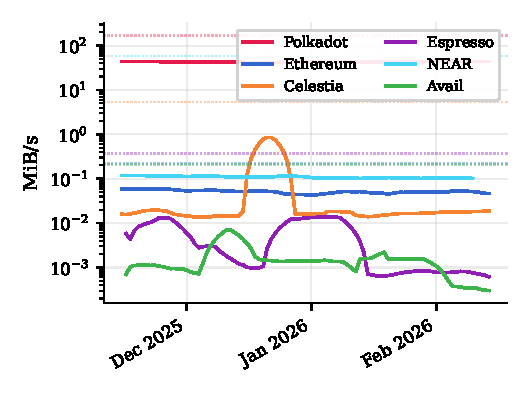
\includegraphics[width=\textwidth]{cross_throughput.pdf}
        \caption{Throughput (MiB/s, 7-day mean, log scale)}
    \end{subfigure}\hfill
    \begin{subfigure}[b]{0.49\textwidth}
        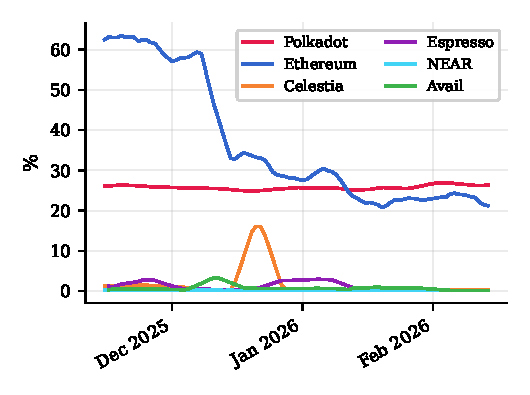
\includegraphics[width=\textwidth]{cross_utilization.pdf}
        \caption{Utilization (\%, 7-day mean)}
    \end{subfigure}

    \vspace{0.2cm}
    \begin{subfigure}[b]{0.49\textwidth}
        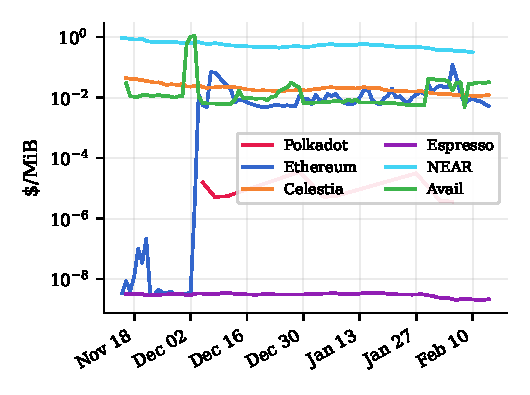
\includegraphics[width=\textwidth]{cross_cost.pdf}
        \caption{Median cost (\$/MiB, log scale)}
    \end{subfigure}\hfill
    \begin{subfigure}[b]{0.49\textwidth}
        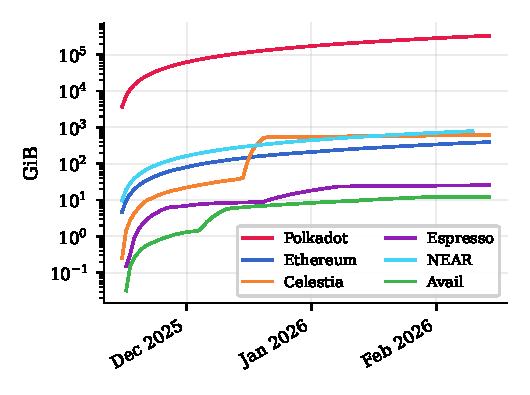
\includegraphics[width=\textwidth]{cross_cumulative.pdf}
        \caption{Cumulative volume (GiB, log scale)}
    \end{subfigure}
    \caption{Cross-protocol comparison over the 90-day window.
    All protocols operate well below their capacity ceilings; Celestia's December~16--21 surge peaks at $\sim$22\% of its (quadrupled) capacity.
    Polkadot throughput and volume are upper bounds (Section~\ref{sec:meth-normalization}).}
    \label{fig:cross}
\end{figure*}

\begin{table}[t]
\centering
\caption{90-day throughput and utilization summary.}
\label{tab:throughput_summary}
\setlength{\tabcolsep}{3pt}
\footnotesize
\begin{tabular}{lcccc}
\toprule
\textbf{Protocol} & \textbf{Max MiB/s} & \textbf{p50 MiB/s} & \textbf{Mean MiB/s} & \textbf{Mean util.} \\
\midrule
Polkadot & $\sim$167 & $\sim$42.8$^\dagger$ & $\sim$43.0$^\dagger$ & $\sim$25.8\% \\
Ethereum & 0.22 & $\sim$0.051 & $\sim$0.051 & $\sim$35\% \\
Celestia & 1.33$\to$5.31 & $\sim$0.018 & $\sim$0.024 & $\sim$1.7\% \\
Espresso & 0.37 & $\sim$0.002 & $\sim$0.003 & $\sim$1.5\% \\
NEAR & $\sim$59 & $\sim$0.107 & $\sim$0.108 & $\sim$0.18\% \\
Avail & 0.21 & $\sim$0.001 & $\sim$0.002 & $<$1\% \\
\bottomrule
\end{tabular}

\vspace{2pt}
\raggedright\footnotesize{$^\dagger$Upper bound: assumes max PoV size per included candidate. Ethereum and Celestia utilization is against the maximum in force on each day.}
\end{table}

Key observations:
\begin{enumerate}
    \item \textbf{Universal under-utilization.} No protocol's mean utilization exceeds 40\%. Polkadot is stable at $\sim$25--27\% ($\sim$26 of 100 cores engaged per day). Ethereum has the highest sustained utilization: $\sim$60\% under Pectra and Fusaka, falling to $\sim$31\% after BPO1 and $\sim$23\% after BPO2 as capacity grew faster than demand. Celestia runs at $\le$1\% in steady state, NEAR at $\sim$0.18\% despite $\sim$9~GiB/day of payload, and Espresso and Avail at a few percent at most.
    \item \textbf{Demand, not supply.} Because all protocols are demand-constrained, observed throughput reflects ecosystem adoption rather than engineering limits; raw MiB/s comparisons measure market share, not capability.
    \item \textbf{NEAR's volume paradox.} NEAR has the lowest utilization but the second-highest volume ($\sim$833~GiB over the window, after Polkadot's upper-bound $\sim$340~TiB; Ethereum $\sim$392~GiB; Celestia $\sim$200~GiB), because its $\sim$59~MiB/s capacity across 9~shards far exceeds demand.
\end{enumerate}

\subsection{Cost Analysis}
\label{sec:results-cost}

Fig.~\ref{fig:cost_quantiles} shows per-protocol daily cost quantile bands (p10/p50/p90) and Table~\ref{tab:cost_summary} summarizes the distributions.

\begin{figure*}[t]
    \centering
    \begin{subfigure}[b]{0.32\textwidth}
        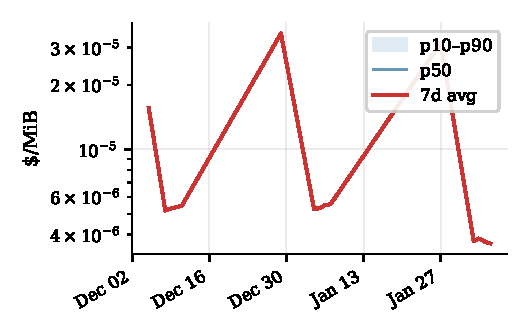
\includegraphics[width=\textwidth]{polkadot_cost.pdf}
        \caption{Polkadot}
    \end{subfigure}\hfill
    \begin{subfigure}[b]{0.32\textwidth}
        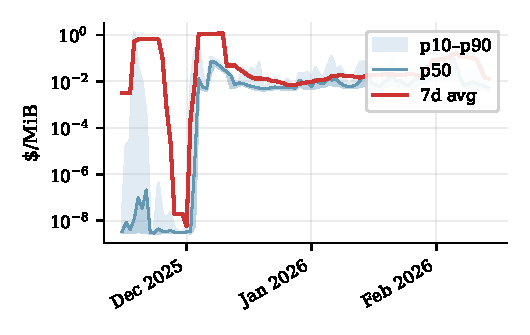
\includegraphics[width=\textwidth]{eth_cost.pdf}
        \caption{Ethereum}
        \label{fig:cost_q_eth}
    \end{subfigure}\hfill
    \begin{subfigure}[b]{0.32\textwidth}
        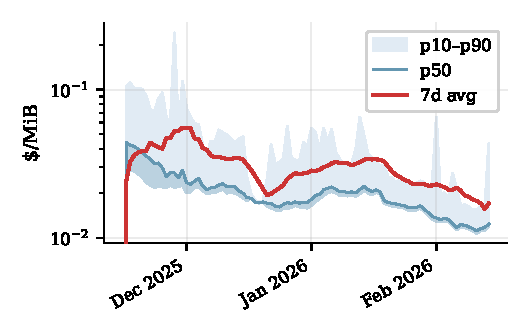
\includegraphics[width=\textwidth]{celestia_cost.pdf}
        \caption{Celestia}
    \end{subfigure}

    \vspace{0.2cm}
    \begin{subfigure}[b]{0.32\textwidth}
        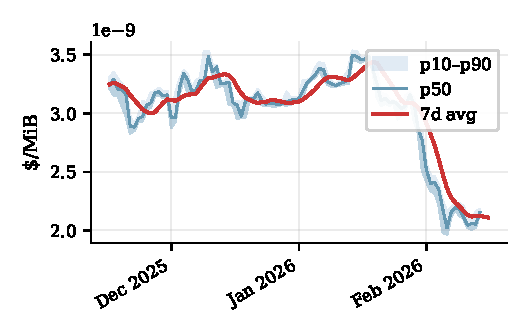
\includegraphics[width=\textwidth]{espresso_cost.pdf}
        \caption{Espresso}
    \end{subfigure}\hfill
    \begin{subfigure}[b]{0.32\textwidth}
        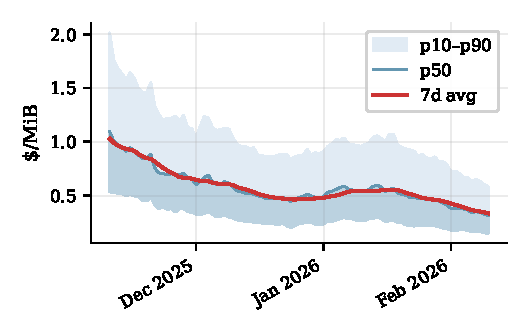
\includegraphics[width=\textwidth]{near_cost.pdf}
        \caption{NEAR}
    \end{subfigure}\hfill
    \begin{subfigure}[b]{0.32\textwidth}
        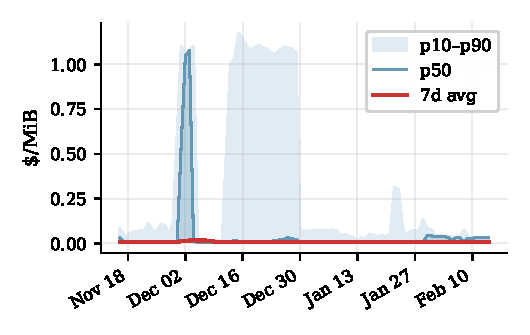
\includegraphics[width=\textwidth]{avail_cost.pdf}
        \caption{Avail}
    \end{subfigure}
    \caption{Daily cost quantile bands (\$/MiB) per protocol.
    (a)~Polkadot bulk coretime, on days with purchases only.
    (b)~Ethereum: fees sit at the 1-wei floor until Fusaka (Dec~3), then settle near \$0.005--0.02/MiB.
    (c)~Celestia declines from $\sim$\$0.05 to $\sim$\$0.02/MiB, partly with the TIA price.
    (d)~Espresso's fixed 1~wei/byte fee tracks ETH/USD.
    (e)~NEAR has the highest median among active fee markets.
    (f)~Avail has the widest spread, with p50 spikes above \$1/MiB.}
    \label{fig:cost_quantiles}
\end{figure*}

\begin{table}[t]
\centering
\caption{90-day cost summary (\$/MiB).}
\label{tab:cost_summary}
\setlength{\tabcolsep}{2.5pt}
\footnotesize
\begin{tabular}{lccccc}
\toprule
\textbf{Protocol} & \textbf{p50} & \textbf{p90} & \textbf{p99} & \textbf{VWAP} & \textbf{Pricing} \\
\midrule
Polkadot & 5.3$\times$10$^{-6}$$^\ast$ & 2.7$\times$10$^{-5}$ & 3.5$\times$10$^{-5}$ & --- & Coretime \\
Ethereum & 7.3$\times$10$^{-3}$ & 0.023 & 0.074 & 0.18 & Blob gas \\
Celestia & 0.020 & 0.030 & 0.042 & 0.025 & Gas/byte \\
Espresso & 3.1$\times$10$^{-9}$ & 3.4$\times$10$^{-9}$ & 3.5$\times$10$^{-9}$ & 3.1$\times$10$^{-9}$ & Fixed fee \\
NEAR & 0.53 & 0.71 & 0.92 & 0.54 & Gas \\
Avail & 0.0096 & 0.032 & 1.05 & 0.0074 & Fee+modifier \\
\bottomrule
\end{tabular}

\vspace{2pt}
\raggedright\footnotesize{$^\ast$Sparse: 14 of 94 days had bulk coretime purchases; amortized over max PoV capacity. Quantiles are over the distribution of daily median costs in the window for every protocol; VWAP is total DA spend divided by total DA volume.}
\end{table}

Key findings:
\begin{enumerate}
    \item \textbf{More than eight orders of magnitude.} Median DA cost ranges from $\sim$\$3$\times$10$^{-9}$/MiB (Espresso) to $\sim$\$0.53/MiB (NEAR). The range reflects different economic designs, not only protocol efficiency.
    \item \textbf{Espresso's cost is not an economic signal.} The fee has been fixed at 1~wei/byte since genesis, so its curve mirrors ETH/USD (falling from $\sim$\$3.5$\times$10$^{-9}$ to $\sim$\$2$\times$10$^{-9}$ as ETH fell). This is a permissioned Mainnet~0 artifact, not a fee market.
    \item \textbf{Ethereum's floor exit is driven by EIP-7918, not by BPO demand.} Before Fusaka the blob base fee sat at the 1-wei floor for $\sim$28\% of blocks and the median cost was $\sim$\$4$\times$10$^{-9}$/MiB. From the first post-Fusaka day the floor share drops to zero and median cost jumps six orders of magnitude to $\sim$\$0.009/MiB, before BPO1 adds any capacity (Section~\ref{sec:results-upgrades}).
    \item \textbf{Avail has the widest spread.} Its median (\$0.0096/MiB) is comparable to Celestia's, but its p99 reaches $\sim$\$1.05 during brief activity surges around December~4 and late December, suggesting the fee modifier amplifies volatility even at low throughput.
    \item \textbf{NEAR has the highest meaningful cost}, declining from $\sim$\$0.75 to $\sim$\$0.30/MiB over the window, reflecting gas pricing applied to encoded receipt data.
    \item \textbf{Polkadot's cost is sparse but negligible}, because coretime bundles execution and DA; the DA component is effectively a by-product of core acquisition.
\end{enumerate}

\subsubsection{Retention-Adjusted Cost}
Table~\ref{tab:annualized_cost} and Fig.~\ref{fig:landscape}(b) normalize cost by retention (Section~\ref{sec:meth-metrics}).

\begin{table}[t]
\centering
\caption{Annualized DA cost, accounting for retention.}
\label{tab:annualized_cost}
\setlength{\tabcolsep}{4pt}
\begin{tabular}{lccc}
\toprule
\textbf{Protocol} & \textbf{Retention} & \textbf{Reposts/yr} & \textbf{p50 \$/MiB/yr} \\
\midrule
NEAR & $\sim$1.5\,d & $\sim$243 & $\sim$129 \\
Celestia & 7\,d & $\sim$52 & $\sim$1.0 \\
Ethereum & $\sim$18\,d & $\sim$20 & $\sim$0.15 \\
Polkadot & 25\,h & $\sim$350 & $\sim$0.002 \\
Avail & node-set & --- & (spot 0.0096) \\
Espresso & node-set & --- & (spot 3$\times$10$^{-9}$) \\
\bottomrule
\end{tabular}
\end{table}

Short retention multiplies cost: NEAR's 5-epoch garbage-collection window ($\sim$1.5~days) requires $\sim$243 reposts per year and gives by far the highest annualized cost ($\sim$\$129/MiB/yr), while Celestia's 7-day sampling window lifts its \$0.02/MiB spot cost to $\sim$\$1/MiB/yr.
Ethereum's 18-day window keeps its annualized cost near \$0.15/MiB/yr, and Polkadot's cost stays negligible even after $\sim$350 reposts.
Avail and Espresso define no protocol-level expiry, so their cost cannot be annualized on the same basis.

\begin{figure*}[t]
    \centering
    \begin{subfigure}[b]{0.49\textwidth}
        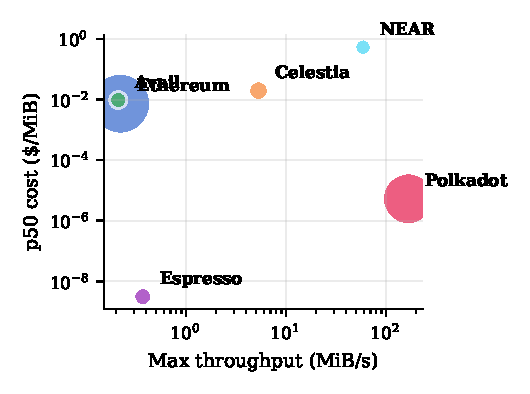
\includegraphics[width=\textwidth]{cross_capacity_vs_cost.pdf}
        \caption{Maximum throughput vs.\ median cost (bubble size: mean utilization)}
    \end{subfigure}\hfill
    \begin{subfigure}[b]{0.49\textwidth}
        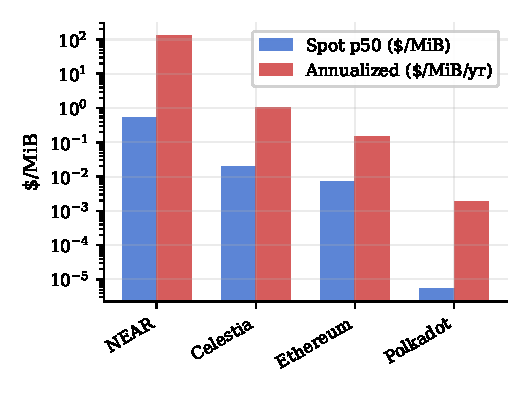
\includegraphics[width=\textwidth]{cross_retention_adjusted_cost.pdf}
        \caption{Spot vs.\ annualized cost}
    \end{subfigure}
    \caption{DA protocol landscape. Protocols cluster by design philosophy rather than along a single capacity--cost frontier, and retention reorders the cost ranking.}
    \label{fig:landscape}
\end{figure*}

\subsection{Natural Experiments: Protocol Upgrades}
\label{sec:results-upgrades}

\subsubsection{Ethereum: Pectra $\rightarrow$ Fusaka $\rightarrow$ BPO1 $\rightarrow$ BPO2}

Fig.~\ref{fig:eth} separates the effect of Ethereum's three upgrades.
\squishlist
    \item \textbf{Fusaka (fee floor).} Under Pectra the blob fee was at the 1-wei minimum for 5--68\% of blocks per day. Fusaka's EIP-7918 ties a reserve price to the execution base fee; from December~4 no block is at the floor (Fig.~\ref{fig:eth}(c)) and median cost rises to $\sim$\$0.009/MiB, while utilization is unchanged ($\sim$58\%).
    \item \textbf{BPO1 and BPO2 (capacity).} Each capacity step lowered utilization (from $\sim$58\% to $\sim$31\% to $\sim$23\%) and target utilization (from $\sim$87\% to $\sim$47\% to $\sim$34\%; Fig.~\ref{fig:eth}(b)). Median cost stayed in a narrow \$0.007--0.010/MiB band across both BPO eras (Fig.~\ref{fig:eth}(a)), consistent with fees held near the EIP-7918 reserve price rather than set by congestion.
    \item \textbf{Demand.} Daily blob volume stayed at $\sim$4.1--4.7~GiB/day across all four eras, so the added capacity has not yet been absorbed.
\squishend

\begin{figure*}[t]
    \centering
    \begin{subfigure}[b]{0.32\textwidth}
        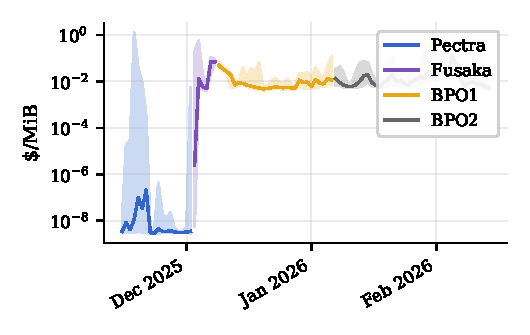
\includegraphics[width=\textwidth]{eth_cost_eras.pdf}
        \caption{Cost bands by era (\$/MiB)}
    \end{subfigure}\hfill
    \begin{subfigure}[b]{0.32\textwidth}
        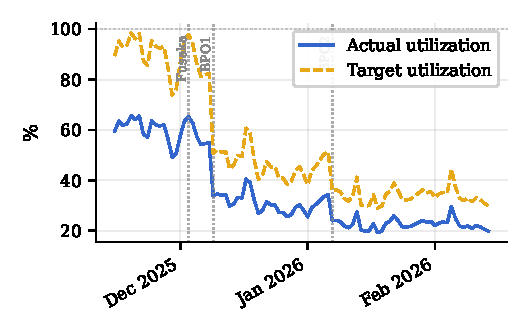
\includegraphics[width=\textwidth]{eth_target_vs_actual.pdf}
        \caption{Target vs.\ actual utilization (\%)}
    \end{subfigure}\hfill
    \begin{subfigure}[b]{0.32\textwidth}
        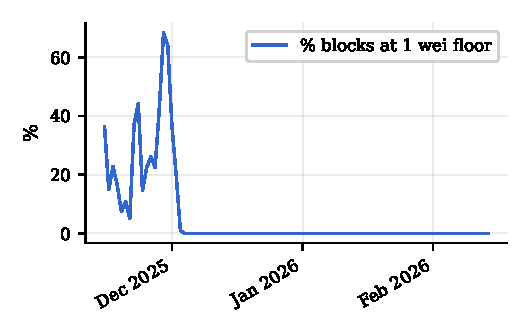
\includegraphics[width=\textwidth]{eth_pct_at_floor.pdf}
        \caption{Blocks at the 1-wei fee floor (\%)}
    \end{subfigure}
    \caption{Ethereum blob market across the Pectra, Fusaka, BPO1 and BPO2 eras. The fee leaves the floor at Fusaka (EIP-7918), before any capacity change; the BPO forks lower utilization without materially changing median cost.}
    \label{fig:eth}
\end{figure*}

\subsubsection{Celestia: December Demand Surge}

Celestia raised its maximum square from 128 to 256 on December~3, quadrupling capacity to $\sim$5.3~MiB/s.
From December~16 to~21, daily throughput rose eighty-fold, from a baseline of $\sim$0.015~MiB/s to $\sim$1.2~MiB/s. That is $\sim$22\% of the new ceiling, but it would have saturated the pre-December capacity of 1.33~MiB/s.
Cost did \emph{not} rise: the daily median fell slightly (\$0.020 to \$0.017/MiB) and the p90 collapsed onto the median, indicating that the surge consisted of large blobs posted at the minimum gas price rather than competing demand. Afterwards throughput and the p90 returned to their pre-event levels.
The episode shows capacity being added ahead of demand: the largest demand event in our window did not exercise the fee market.

\subsection{Block Dynamics and Polkadot Core Engagement}
\label{sec:results-blocks}

Fig.~\ref{fig:blocks}(a--b) shows block time distributions for the two protocols where they are informative; fixed-cadence protocols (Ethereum 12\,s, Polkadot 6\,s, Avail 20\,s) are trivially tight.
Celestia holds 5--6\,s after an elevated p90 in mid-November.
Espresso's responsive HotShot consensus has p10~$\sim$1\,s and p50~$\sim$2\,s, with a p90 that falls from $\sim$6.5\,s in the first weeks to $\sim$3\,s by February.

Fig.~\ref{fig:blocks}(c) shows that only $\sim$26 of 100 Polkadot cores were engaged on a typical day, leaving $\sim$74\% idle capacity: the relay chain could host roughly three times as many parachains at current PoV sizes without parameter changes.

\begin{figure*}[t]
    \centering
    \begin{subfigure}[b]{0.32\textwidth}
        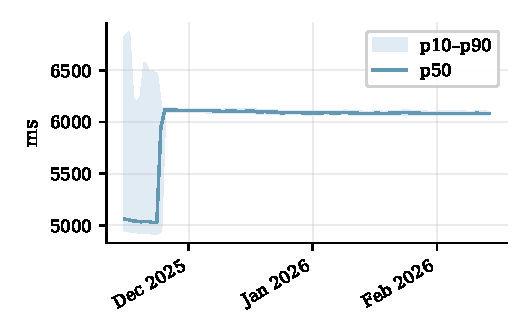
\includegraphics[width=\textwidth]{celestia_blocktime.pdf}
        \caption{Celestia block time (ms)}
    \end{subfigure}\hfill
    \begin{subfigure}[b]{0.32\textwidth}
        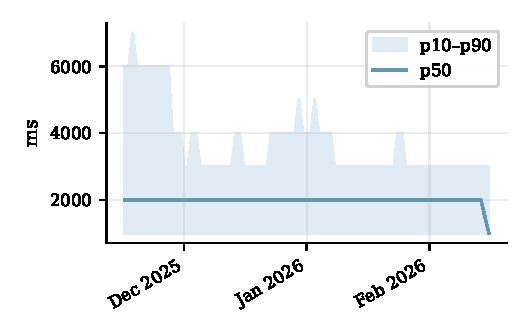
\includegraphics[width=\textwidth]{espresso_blocktime.pdf}
        \caption{Espresso block time (ms)}
    \end{subfigure}\hfill
    \begin{subfigure}[b]{0.32\textwidth}
        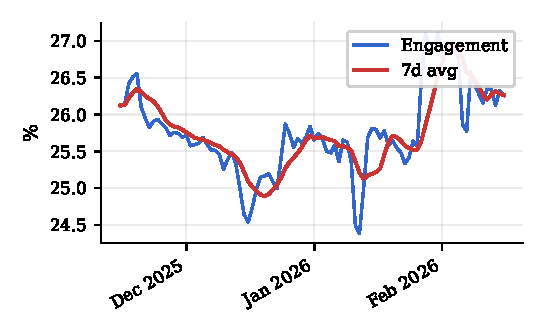
\includegraphics[width=\textwidth]{polkadot_core_engagement.pdf}
        \caption{Polkadot core engagement (\%)}
    \end{subfigure}
    \caption{Block time distributions (p10/p50/p90) for Celestia and Espresso, and Polkadot core engagement.}
    \label{fig:blocks}
\end{figure*}

Espresso's payload pattern (two burst periods in November and late December--early January, then collapse to $<$50~MiB/day) suggests non-organic traffic typical of an early permissioned deployment, in contrast to Celestia's sustained 30--100~MiB/hour baseline.


\section{Security and Trust Analysis}
\label{sec:security}
% ================================================================
% SECTION VI: SECURITY AND TRUST ANALYSIS
% ================================================================

This section analyzes the security properties and trust assumptions of each DA protocol, focusing on Byzantine fault tolerance, data withholding enforcement, retention guarantees, and decentralization characteristics.

\subsection{Byzantine Fault Tolerance}
\label{sec:security-bft}

All six protocols inherit the classical BFT bound of $f < n/3$, where $f$ is the number of Byzantine-faulty nodes and $n$ is the total committee or validator set size.
However, the practical manifestation of this threshold varies substantially.

\paragraph{Polkadot}
Polkadot's relay chain requires $\geq 2/3$ of validators to sign availability bitfields before a parachain block can be included and finalized.
With approximately 600~active validators, the system tolerates up to $\sim$200 Byzantine faults.
The ELVES protocol further strengthens this through approval checking: randomly selected validators re-execute parachain blocks post-inclusion, and a single invalid execution triggers a dispute that can slash the responsible validators~\cite{Jeff_Burdges_ELVES}.
The probability of an invalid block escaping detection decreases exponentially with the number of approval checkers.

\paragraph{Ethereum}
Ethereum's Casper FFG requires a $2/3$ supermajority of validators (by stake weight) to finalize blocks.
With approximately 1~million active validators, the economic security backing finality exceeds \$30~billion (at ETH $\sim$\$3,000).
PeerDAS distributes custody across the validator set: each validator holds a subset of blob columns, and system-level availability confidence emerges from the aggregate custody distribution~\cite{EIP-7594}.
The large validator set makes coordinated withholding attacks economically prohibitive.

\paragraph{Celestia}
Celestia runs CometBFT (Tendermint) consensus, which requires $\geq 2/3$ of validators (by stake weight) to commit each block.
The validator set is capped at 100 in the current configuration.
DAS provides an additional layer of security: even if validators finalize a block with unavailable data, light client sampling will probabilistically detect the withholding~\cite{AlBassam_FraudDA}.
This two-layer model (consensus BFT + sampling) provides stronger guarantees than consensus alone, at the cost of requiring sufficient light client participation.

\paragraph{Espresso}
Espresso's HotShot consensus operates with 100~nodes across 20~operators in the Mainnet~0 configuration.
The DA certificate requires $\geq 2/3$ of committee signatures, tolerating up to $\sim$33 Byzantine nodes.
However, the small operator count (20) means that the effective trust assumption is closer to $f < 7$ at the operator level~\cite{Espresso:Hotshot_and_Triamisu}.

\paragraph{NEAR}
NEAR's Nightshade sharding applies the BFT threshold per shard.
With 9~shards and approximately 400~validators, the per-shard committee size depends on stake distribution.
A critical assumption is that each shard independently maintains $< 1/3$ Byzantine nodes; an adversary who concentrates stake in a single shard can potentially compromise that shard's DA at lower total cost than compromising the network-wide threshold~\cite{NEAR_Nightshade_Scaling_Blockchain}.
In practice, however, most mainnet validators currently track all shards rather than only their assigned shard, which means the per-shard BFT assumption is more theoretical than operational: DA benefits from full-network replication even though the protocol is designed for shard-local storage.

\paragraph{Avail}
Avail's BABE/GRANDPA consensus requires $\geq 2/3$ honest validators for both block production and finality.
DAS light clients provide independent verification, analogous to Celestia's model.
The VectorX bridge to Ethereum introduces an additional trust surface: bridge liveness depends on the prover infrastructure, and the approximately 2-hour bridge delay creates a window during which Avail-native finality and Ethereum-bridged attestations may diverge~\cite{Avail_The_DA_Blockchain}.

Table~\ref{tab:bft_comparison} summarizes the BFT characteristics across protocols.

\begin{table*}[t]
\centering
\caption{Byzantine Fault Tolerance and Validator Set Characteristics}
\label{tab:bft_comparison}
\setlength{\tabcolsep}{3pt}
\footnotesize
\begin{tabular}{lccccc}
\toprule
\textbf{Protocol} & \textbf{BFT Threshold} & \textbf{Validator Count} & \textbf{Consensus} & \textbf{Finality} & \textbf{Stake} \\
\midrule
Polkadot & $f < n/3$ & $\sim$600 & BABE + GRANDPA & 12--60\,s & $\sim$1.8M DOT min \\
Ethereum & $f < n/3$ (stake) & $\sim$1M & Casper FFG & $\sim$12.8\,min & 32 ETH per validator \\
Celestia & $f < n/3$ (stake) & $\sim$100 & CometBFT & Single-slot ($\sim$6\,s) & Variable \\
Espresso & $f < n/3$ & 100 (20 operators) & HotShot & $\sim$1--2\,s & None (permissioned) \\
NEAR & $f < n/3$ per shard & $\sim$400 & Nightshade & $\sim$2\,s & Seat-price auction \\
Avail & $f < n/3$ & $\sim$100 & BABE + GRANDPA & 20--60\,s & Variable \\
\bottomrule
\end{tabular}
\end{table*}

\subsection{Data Withholding Enforcement}
\label{sec:security-withholding}

As established in Section~\ref{subsec:verification}, no protocol implements slashing specifically for data withholding.
Here we analyze the indirect enforcement mechanisms and their practical effectiveness.

Detection is sampling-based for Celestia, Avail and Ethereum (missing responses to random samples), attestation-based for Polkadot and NEAR (a missing bitfield or chunk endorsement is visible on-chain, but only validator-level withholding is detected), and certificate-based for Espresso (a missing DA certificate blocks finalization).

\paragraph{Enforcement gap}
The fundamental challenge across all protocols is the \emph{attribution gap}: detecting that data is unavailable does not identify the responsible party.
A validator that fails to serve a chunk may be offline, network-partitioned, or maliciously withholding, and the protocol cannot distinguish these cases.
This attribution difficulty explains why no protocol has implemented withholding-specific slashing: the false positive rate (slashing honest nodes experiencing network issues) would be unacceptable.

\subsection{Retention and Persistence}
\label{sec:security-retention}

No protocol guarantees permanent availability (Table~\ref{tab:feature_comparison}). Four define a window: Polkadot's availability store keeps finalized chunks for 25~hours, NEAR garbage-collects after 5~epochs ($\sim$1.5~days), Celestia light nodes sample within 7~days (CIP-036), and Ethereum serves blobs for 4{,}096~epochs ($\sim$18~days). Avail and Espresso define no network-wide expiry: Avail nodes keep block data by default and Espresso nodes choose their own pruning policy, so availability beyond the latest blocks rests on operators rather than the protocol.
This variation has critical implications for rollup security:

\begin{itemize}
    \item \textbf{Fraud proof windows}: Optimistic rollups require a challenge period (typically 7~days) during which fraud proofs can be submitted; the DA layer must retain data at least as long as the challenge period. Polkadot (25~h) and NEAR ($\sim$1.5~d) retain data for less than the standard 7-day fraud-proof window, and Celestia's 7-day sampling window leaves no margin, so rollups must archive data externally or shorten challenge periods; on Avail and Espresso, retention depends on node configuration.

    \item \textbf{Bridging latency}: Cross-chain bridges that verify DA attestations must complete verification within the retention window. Avail's VectorX bridge to Ethereum has an approximately 2-hour attestation delay, during which Avail-native finality and Ethereum-side attestations diverge.

    \item \textbf{Archival burden}: After DA expiry, data persistence shifts to voluntary archival by full nodes, third-party indexers, or rollup operators themselves. No protocol guarantees post-retention data retrievability.
\end{itemize}

\subsection{Trust Assumptions Summary}
\label{sec:security-trust}

Table~\ref{tab:trust_summary} maps each protocol's key trust assumptions.

\begin{table*}[t]
\centering
\caption{Trust Assumption Comparison Across DA Protocols}
\label{tab:trust_summary}
\setlength{\tabcolsep}{4pt}
\renewcommand{\arraystretch}{1.2}
\footnotesize
\begin{tabular}{p{1.4cm}p{4.9cm}p{4.9cm}p{4.9cm}}
\toprule
\textbf{Protocol} & \textbf{Availability Assumption} & \textbf{Encoding Trust} & \textbf{Additional Assumptions} \\
\midrule
Polkadot & $\geq 2/3$ validators honest (bitfield voting) & Validators re-encode and verify (approval checking) & Relay chain liveness \\
Ethereum & $\geq 2/3$ validators honest (Casper FFG) + sufficient custody distribution & KZG algebraic verification (no fraud proofs needed) & Trusted setup integrity (KZG ceremony) \\
Celestia & $\geq 2/3$ validators honest + sufficient DAS participation & BEFPs from $\geq 1$ honest full node & $\geq 1$ non-eclipsed honest full node \\
Espresso & $\geq 2/3$ committee signs DA certificate & KZG + vector commitment algebraic verification & Committee honesty; CDN liveness \\
NEAR & $< 1/3$ Byzantine per shard & Chunk producers re-encode & Honest shard assignment; no stake concentration \\
Avail & $\geq 2/3$ validators honest + DAS participation & KZG algebraic verification & Trusted setup integrity; VectorX bridge liveness \\
\bottomrule
\end{tabular}
\end{table*}

The trust models fall into three categories.
\emph{DAS-enhanced protocols} (Celestia, Avail, Ethereum) provide the strongest light client guarantees but require active network participation in sampling.
\emph{Validator-recovery protocols} (Polkadot, NEAR) provide deterministic guarantees conditioned on validator honesty but offer no independent light client verification.
\emph{VID-based protocols} (Espresso) provide algebraic guarantees against bribery but depend on committee and fallback infrastructure availability.


\section{Discussion}
\label{sec:discussion}
% ================================================================
% SECTION VII: DISCUSSION
% ================================================================

\subsection{Trade-offs Between the Three Paradigms}
\label{sec:disc-paradigms}

\paragraph{DAS protocols (Celestia, Avail, Ethereum)}
These give light clients the strongest guarantees, because a resource-constrained node can check availability itself.
The guarantee weakens if too few nodes sample, a dependence the other two paradigms do not have.

\paragraph{Validator-recovery protocols (Polkadot, NEAR)}
Polkadot's finality gate (GRANDPA will not finalize blocks without sufficient availability bitfields) is the most direct enforcement we observe: unavailable data cannot be finalized.
In exchange, light clients cannot verify availability themselves.
For parachain validation this is acceptable, because the relay chain validators are the main consumers of the data; an external rollup using Polkadot or NEAR for DA would have to trust the validator set.

\paragraph{VID protocol (Espresso)}
None of the other protocols has an equivalent of Tiramisu's algebraic bribery resistance, but in Mainnet~0 it counts for little while the operator set is permissioned (20~operators) and there is no slashing.
The 1~wei/byte fee is likewise a placeholder.
Whether VID's advantages matter in practice will depend on a permissionless deployment with economic security behind it.

\subsection{The Cost--Throughput Frontier}
\label{sec:disc-frontier}

Fig.~\ref{fig:landscape}(a) plots median cost against protocol maximum throughput, and there is no simple inverse relationship.
Espresso combines low cost with moderate throughput, but its cost is a Mainnet~0 placeholder.
Celestia and Avail have moderate throughput at moderate cost.
Polkadot has the highest theoretical throughput ($\sim$167~MiB/s) at $\sim$\$5$\times$10$^{-6}$/MiB, although coretime pays for execution as well as DA.
NEAR combines high capacity ($\sim$59~MiB/s) with the highest cost among active fee markets ($\sim$\$0.53/MiB), the opposite corner from Polkadot.
After Fusaka, Ethereum offers modest capacity at a cost comparable to Celestia and Avail, with the largest validator set and stake behind it.

The protocols were built for different jobs: Polkadot for parachain validation, NEAR for general smart-contract execution, Ethereum for censorship resistance and economic security, and Celestia and Avail as dedicated DA layers.
Cost and throughput therefore do not rank them on their own; retention, trust assumptions, light-client verification and ecosystem integration matter as much.

\subsection{Polkadot's Scaling Headroom}
\label{sec:disc-polkadot}
With only $\sim$26 of 100 cores engaged (Fig.~\ref{fig:blocks}(c)), Polkadot has $\sim$74\% idle DA capacity: throughput could grow from the current upper bound of $\sim$43~MiB/s toward $\sim$167~MiB/s without parameter changes.
As engagement rises, the coretime market should raise core prices; at the current $\sim$\$5$\times$10$^{-6}$/MiB, cost is unlikely to limit near-term growth.
Because actual PoV sizes are not exposed on-chain, a more precise capacity analysis requires PoV-level data.

\subsection{Implications for Rollup Developers}
\label{sec:disc-rollups}

Retention constrains a rollup's choice of DA layer before cost does.
An optimistic rollup with a 7-day challenge period cannot rely on Polkadot (25~h) or NEAR ($\sim$1.5~d) without its own archive, and Celestia's 7-day sampling window leaves no margin.
For the same reason, spot prices mislead on short-retention layers; the annualized cost (Section~\ref{sec:meth-metrics}) counts the reposts needed to keep data available.
Fee floors and token prices, more than congestion, currently set what rollups pay: Ethereum's post-Fusaka cost sits near the EIP-7918 reserve price, and Celestia's largest demand surge did not raise its median fee.
With every protocol below 40\% mean utilization, capacity does not yet separate the options; how fee markets behave under load will matter once utilization rises.

\subsection{Protocol Design Observations}
\label{sec:disc-design}

\paragraph{Withholding enforcement}
No protocol can attribute withholding to a specific actor, which suggests that slashing for omission faults is harder than slashing for commission faults such as equivocation or invalid execution.
Other enforcement models may be needed, for example insurance schemes, reputation systems with gradual stake reduction, or cryptographic mechanisms that make withholding unprofitable without having to attribute it.

\paragraph{Retention}
Four protocols define an expiry window, and Avail and Espresso leave retention to node operators.
This is by design: keeping all history indefinitely does not scale, and a DA layer exists to provide a window for verification and fraud detection.
Rollups and applications that need data beyond that window must store it elsewhere, for example on IPFS, Filecoin or Arweave.

\paragraph{Redundancy and commitments}
Among these six protocols, higher redundancy goes with simpler commitments.
Celestia (4$\times$) uses NMTs and Polkadot and NEAR (3$\times$) use Merkle trees, while Ethereum and Avail (2$\times$) use KZG, which verifies encoding without fraud proofs.
Espresso's polynomial VID also relies on algebraic commitments, which provide encoding verification and bribery resistance at a configurable redundancy.

\subsection{Limitations and Threats to Validity}
\label{sec:disc-limitations}

\paragraph{Demand-constrained measurements}
Observed throughput reflects demand during one 90-day window; conclusions about maximum throughput must come from protocol parameters (Section~\ref{sec:meth-normalization}).

\paragraph{Token prices}
USD costs depend on token prices, which moved widely during the window (ETH roughly \$2,000--\$4,000, TIA \$0.30--\$0.85), so another window would give different figures.
Reporting VWAP and percentiles reduces this effect but does not remove it.

\paragraph{Polkadot throughput upper bound}
Polkadot throughput is an upper bound because PoV sizes are not exposed on-chain; parachains typically use 1--3~MiB of the 10~MiB maximum.

\paragraph{Espresso Mainnet~0}
Mainnet~0 is a permissioned early deployment, so its cost, throughput and security figures cannot be compared on equal terms with permissionless, economically secured networks.
We include it for architectural completeness.

\paragraph{Single observation window}
A 90-day window is a snapshot, and behaviour under other market conditions, governance events or adoption levels may differ.
The released tooling can be used to extend the window.

\paragraph{Cross-protocol normalization}
Converting blob gas, coretime, gas and fixed fees to \$/MiB hides some economic detail: Polkadot's coretime also buys execution, and NEAR's gas price covers general contract execution.
The retention-adjusted cost (Table~\ref{tab:annualized_cost}, Fig.~\ref{fig:landscape}(b)) addresses part of this, but no single metric captures all of it.


\section{Conclusion}
\label{sec:conclusion}
% ================================================================
% SECTION VIII: CONCLUSION
% ================================================================

We measured six production DA protocols (Polkadot ELVES, Ethereum EIP-4844/PeerDAS, Celestia, Espresso Tiramisu, NEAR and Avail) with one methodology, using 90~days of mainnet data covering over 14~million blocks.

\subsection{Summary of Findings}

Every protocol's mean utilization was below 40\%.
The networks are demand-constrained, so until they approach saturation, cross-protocol throughput comparisons measure adoption.

Median DA cost spans more than eight orders of magnitude, from $\sim$\$3$\times$10$^{-9}$/MiB (Espresso, whose 1~wei/byte fee is a Mainnet~0 placeholder) to $\sim$\$0.53/MiB (NEAR).
On Ethereum, the blob fee left the 1-wei floor because of Fusaka's EIP-7918 reserve price, before the BPO forks added capacity.
Annualizing cost over each protocol's retention window shows that a protocol that is cheap at spot can be expensive when data must stay available.

No protocol slashes for pure data withholding.
Polkadot gates finality on availability bitfields, Celestia uses bad-encoding fraud proofs, Ethereum uses peer scoring, Espresso relies on committee reputation, NEAR has an unused challenge mechanism, and Avail slashes only for equivocation.
Attributing withholding, an omission fault, to a specific actor is still unsolved.

No protocol guarantees permanent availability.
Protocol-defined retention ranges from 25~hours (Polkadot) to $\sim$18~days (Ethereum), Avail and Espresso leave retention to node operators, and only Ethereum's window comfortably exceeds a 7-day optimistic-rollup challenge period.

\subsection{Future Work}

\emph{Longitudinal extension}: repeating these measurements as utilization rises would show supply-constrained behaviour that the current data cannot.
\emph{Stress testing}: controlled synthetic load would measure protocol limits directly, which observational data cannot do.
\emph{Withholding enforcement}: incentive-compatible enforcement for omission faults needs formal analysis.
\emph{Cross-layer analysis}: measuring end-to-end rollup performance (confirmation time, cost, finality) for each DA backend would show how the choice affects rollups.
\emph{PeerDAS at scale}: PeerDAS activated during our window; its effect on node bandwidth and on further BPO increases is the next thing to measure.


% ================================================================
\section*{CRediT authorship contribution statement}
\textbf{Prasad Kumkar:} Conceptualization, Methodology, Software, Data curation, Formal analysis, Visualization, Writing -- original draft.
\textbf{Pranjal Sarode:} Investigation, Software, Validation, Writing -- review \& editing.


\section*{Declaration of competing interest}
The authors are employed by Chainscore Labs, a blockchain engineering firm. Chainscore Labs develops software in the Polkadot ecosystem, including an implementation of the JAM protocol, and lists the Web3 Foundation, Polkadot and NEAR among its partners. This study was funded by a Web3 Foundation grant (see Funding). All measurements use public mainnet data, and all code and data are openly released so that the results can be independently reproduced. The authors hold ETH and DOT tokens, the native assets of two of the six protocols studied. The authors declare no other known competing financial interests or personal relationships that could have appeared to influence the work reported in this paper.

\section*{Funding}
This work was supported by the Web3 Foundation under the W3F Grants Program. The funder had no role in study design, data collection and analysis, decision to publish, or preparation of the manuscript.

\section*{Data availability}
All collection scripts, datasets and analysis code are publicly available at \url{https://github.com/Chainscore/score-da} and archived on Zenodo (\url{https://doi.org/10.5281/zenodo.23276229}). Code is released under Apache~2.0 and data under CC~BY~4.0.

\section*{Declaration of generative AI and AI-assisted technologies in the manuscript preparation process}
During the preparation of this work the authors used Claude (Anthropic), including Claude Code, in order to assist with writing and reviewing data-collection and analysis scripts, reformatting the manuscript to the journal template, verifying bibliographic metadata, and editing for length. After using this tool, the authors reviewed and edited the content as needed and take full responsibility for the content of the published article.

\bibliographystyle{elsarticle-num}
\bibliography{references}

\end{document}
